% ===================== CORRECT-Error =====================
\subsection{CORRECT-Error}\label{ds:correct_error}
\badgerow{\injected\ \okbadge\ \lbl{agent + step}\ \lbl{MAS (Magentic-One variant)}\ \lbl{GAIA / HotpotQA / MuSiQue / 2Wiki / ARC / MATH-500 / MMLU-Pro}}

\begin{identity}
Paper & \emph{CORRECT: COndensed eRror RECognition via knowledge Transfer in multi-agent systems} --- Yu et al. (UIUC / Amazon), ICML 2026, arXiv:2509.24088 \cite{correct2026}\\
Links & \href{https://huggingface.co/datasets/yifanyu/CORRECT-Error}{HF \code{yifanyu/CORRECT-Error}} \textperiodcentered\ \href{https://github.com/UIUC-MLSys/CORRECT}{GitHub \code{UIUC-MLSys/CORRECT}} \textperiodcentered\ \href{https://www.amazon.science/publications/correct-condensed-error-recognition-via-knowledge-transfer-in-multi-agent-systems}{Amazon Science page}\\
License & Apache-2.0 (dataset card and GitHub \code{LICENSE})\\
Status & downloaded in full, ungated; one parquet file (\code{test} split, 2,226 rows, $\approx$20 MB) plus the GitHub clone (code and pre-extracted error schemata, no trajectories); \code{data/correct\_error/}\\
\end{identity}

\paragraph{Description} CORRECT-Error is the evaluation set released with CORRECT, a training-free attributor that caches distilled ``error schemata'' from past failures and retrieves them to guide an LLM detector. The task is the Who\&When one (\S\ref{ds:who_and_when}): given a failed trajectory, predict \code{mistake\_agent} and \code{mistake\_step}, the earliest step whose correction would have flipped the outcome. All trajectories come from a single MAS---a Magentic-One variant run in AutoGen with selector-group-chat control (roles \code{Planner}, \code{WebSurfer}, \code{Coder}, \code{CodeExecutor}, \code{FileSurfer}; \code{history[0]} is always the \code{user} task message)---on seven task suites (GAIA L1, HotpotQA, MuSiQue, 2WikiMultihopQA, ARC, MATH-500, MMLU-Pro) and two generator LLMs (\code{gpt-5-nano} 1,908, \code{gpt-4o-mini} 318). \textbf{Failures are injected}, not observed: (1) a pool of \emph{successful} trajectories is collected; (2) each is matched by semantic similarity to a human-labelled real failure (the Who\&When Hand-Crafted set) and GPT-5 devises an injection strategy; (3) the generator model rewrites one step into an erroneous action, so the rewritten step is the decisive error by construction (synthesis cost reported at $>$3\,B tokens). \textbf{Validation}: three experts ($>$120\,h) judged a blind mix of synthetic and real failures---47.1\% of synthetic trajectories were taken for human-labelled, 94.4\% were judged genuine by $\ge$2 of 3 labelers; the step labels themselves were not re-checked and no $\kappa$ is reported. Labels are agent + step only: no category, no reason text, no ground-truth answer, and the successful parent trajectories are not released.

\paragraph{Metrics and baselines} Step accuracy with tolerance, Acc@$k$ = $|\text{pred}-\text{gt}|\le k$; agent accuracy is not reported. Paper Table~2, Qwen-2.5-7B detector, \code{gpt-5-nano} subset, Acc@1\,/\,@3\,/\,@5 in \% (paper):

\begin{center}\small
\begin{tabular}{@{}lcc@{}}\toprule
Task & LLM-as-a-Judge & CORRECT\\\midrule
GAIA & 16.7 / 27.8 / 38.9 & 30.6 / 44.4 / 52.8\\
HotpotQA & 14.7 / 48.9 / 65.8 & 35.8 / 72.7 / 84.3\\
MuSiQue & 11.9 / 43.9 / 58.8 & 32.7 / 61.2 / 77.2\\
2Wiki & 6.4 / 35.6 / 56.1 & 16.9 / 49.9 / 69.0\\
ARC & 62.8 / 69.6 / 71.1 & 80.4 / 88.2 / 91.2\\
MATH-500 & 41.8 / 57.1 / 64.3 & 57.1 / 87.8 / 95.9\\
MMLU-Pro & 50.0 / 64.7 / 70.6 & 69.1 / 88.2 / 94.1\\\bottomrule
\end{tabular}
\end{center}
Average gains are +16.8\,/\,+20.1\,/\,+18.9 points on \code{gpt-5-nano} and +20.1\,/\,+27.6\,/\,+28.7 on \code{gpt-4o-mini}; on Who\&When Hand-Crafted, CORRECT lifts Acc@0 from 3.5 to 12.1 (Qwen-2.5-7B). The released \code{src/evaluate.py} scores exact match with a \code{--tolerance} flag.

\paragraph{Schema} One parquet row per trajectory: \code{trajectory\_id} (\code{\{generator\}\_\{dataset\}\_\{question\_id\}}), \code{dataset}, \code{generator\_model}, \code{gaia\_level} (1.0 for the 36 GAIA \code{gpt-5-nano} rows, else null), \code{question}, \code{question\_id} (suffix \code{\_k} indexes injected variants of one source question), \code{history} (list of \{\code{role}, \code{content}\}), \code{mistake\_agent}, \code{mistake\_step} (0-based into \code{history}, user message at 0), \code{mistake\_reason} (empty in every row), \code{groundtruth} (empty), \code{is\_corrected} (always false), \code{level} (always 0).

\paragraph{Statistics} computed from the downloaded parquet.\par\nobreak\vspace{1pt}
\noindent\begin{minipage}[t]{0.48\linewidth}\vspace{0pt}\small
\begin{tabular}{@{}lr@{}}\toprule
trajectories (all failed, one decisive error each) & 2,226\\
by generator: \code{gpt-5-nano} / \code{gpt-4o-mini} & 1,908 / 318\\
distinct source questions (variants per question, max) & 1,440 (1.55, 5)\\
steps: mean / median / min -- max & 11.8 / 10 / 2 -- 22\\
distinct agents (excl.\ user): mean / max & 1.87 / 5\\
error step index: mean / median / max & 5.2 / 5 / 19\\
relative error position: mean / median & 0.69 / 0.95\\
characters / trajectory: mean / median & 27.7\,k / 18.8\,k\\
\code{history[step].role} = \code{mistake\_agent} & 2,040 (91.6\%)\\
rows with \code{mistake\_step} = 0 (user message) & 43\\
non-empty \code{mistake\_reason} / \code{groundtruth} & 0 / 0\\\bottomrule
\end{tabular}

\smallskip By task: 2Wiki 733, HotpotQA 578, MuSiQue 312, ARC 304, MATH-500 157, MMLU-Pro 92, GAIA 50. Length is bimodal: 610 trajectories have $\le$4 steps (ARC/MMLU-Pro, median 2) and 809 have 21--22 steps (MuSiQue median 21), which looks like a round cap. Messages by role: Planner 13.1\,k, WebSurfer 10.6\,k, CodeExecutor 175, Coder 126, FileSurfer 18. Blamed agent: Planner 73.6\%, WebSurfer 21.0\%, \code{Unknown} 42, Coder 23, CodeExecutor 22.
\end{minipage}\hfill
\begin{minipage}[t]{0.50\linewidth}\vspace{0pt}
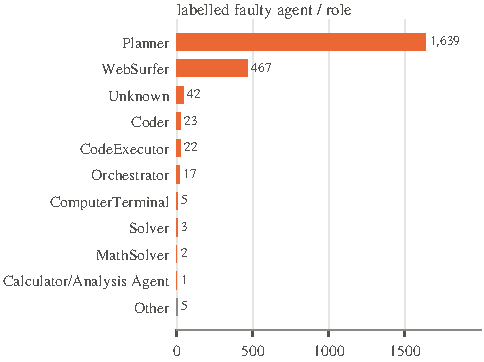
\includegraphics[width=\linewidth]{4_injected/correct_error/figures/agent.pdf}
\end{minipage}

\paragraph{Example trajectory} \code{gpt-5-nano\_gaia\_level1\_task22\_1} (GAIA L1; 8 steps, user + Planner + WebSurfer, 3 roles). The WebSurfer opens the BBC script PDF and sees nothing (step 4); at the injected step 6 it re-opens the same URL and now ``reads'' a scene heading, which the Planner accepts as the final answer. With no \code{groundtruth} and no \code{mistake\_reason} in the release, the error can only be identified as the rewritten step.
% auto-generated by scripts/render_traj.py -- do not edit
\trajtask{gpt-5-nano\_gaia\_level1\_task22\_1}{In Series 9,\allowbreak{} Episode 11 of Doctor Who,\allowbreak{} the Doctor is trapped inside an ever-shifting maze. What is this location called in the official script for the episode?\allowbreak{} Give the setting exactly as it appears in the first scene heading.}
\begin{trajstep}{0}{user}{agA}
You have been given the following task:\allowbreak{}\par In Series 9,\allowbreak{} Episode 11 of Doctor Who,\allowbreak{} the Doctor is trapped inside an ever-shifting maze. What is this location called in the official script for the episode?\allowbreak{} Give the setting exactly as it appears in the first scene heading.\par Available capabilities:\allowbreak{}\newline - WebSurfer:\allowbreak{} Can perform REAL internet searches and browse websites\newline - FileSurfer:\allowbreak{} Can read and analyze files\newline - Coder:\allowbreak{} Can write and analyze code\newline - CodeExecutor:\allowbreak{} Can execute Python code and return results\par Please analyze this task and decide which specialist to engage first. Remember to:\allowbreak{}\newline 1. Break down the task into manageable steps\newline 2. Gather information systematically\newline 3. Build upon previous results\par What is your first action?\allowbreak{}
\end{trajstep}
\begin{trajstep}{1}{Planner}{agB}
**Analysis of Previous Result:\allowbreak{}**\newline No prior results to build on. We're at the information-gathering step to locate the first scene heading from the official Doctor Who script for Series 9,\allowbreak{} Episode 11.\par **Updated Understanding:\allowbreak{}**\newline Task is to identify the exact first scene heading as it appears in the official script for Doctor Who Series 9,\allowbreak{} Episode 11 (the Doctor is in an ever-shifting maze). We must provide the setting exactly as it appears in the first scene heading (including formatting,\allowbreak{} capitalization,\allowbreak{} and punctuation).\par **Decision:\allowbreak{}**\newline - Next Agent:\allowbreak{} WebSurfer\newline - Instructions:\allowbreak{}\newline - Search for the official shooting/\allowbreak{}teleplay script of Doctor Who\newline [...] (639 chars omitted) [...]\newline as it appears,\allowbreak{} and note the source URL next to it. If the heading cannot be found,\allowbreak{} provide the best authoritative alternative and explain any caveats.\par First action:\allowbreak{} Initiate WebSurfer to locate the official script and extract the first scene heading.
\end{trajstep}
\begin{trajstep}{2}{WebSurfer}{agC}
I typed 'Heaven Sent Doctor Who shooting script first scene heading' into the browser search bar.\par The web browser is open to the page [Heaven Sent Doctor Who shooting script first scene heading at DuckDuckGo](https:\allowbreak{}/\allowbreak{}/\allowbreak{}duckduckgo.com/\allowbreak{}?\allowbreak{}q=\allowbreak{}Heaven+Sent+Doctor+Who+shooting+script+first+scene+heading\&ia=\allowbreak{}web).\newline The viewport shows 41\% of the webpage,\allowbreak{} and is positioned at the top of the page\newline The following text is visible in the viewport:\allowbreak{}\par Upgrade to our browser.Try the DuckDuckGo Browser.\newline Fast. Free. Private.Download Browser\newline Free\newline Open menu\newline All\newline Images\newline News\newline Videos\newline More\newline Maps\newline Shopping\newline Search Assist\newline Duck.ai\newline Search Settings\newline Always protected\newline All regions\newline Saf\newline [...] (2,\allowbreak{}506 chars omitted) [...]\newline title":\allowbreak{} "Heaven Sent Doctor Who shooting script first scene heading",\allowbreak{}\newline "viewport":\allowbreak{} "width=\allowbreak{}device-width,\allowbreak{} initial-scale=\allowbreak{}1",\allowbreak{}\newline "HandheldFriendly":\allowbreak{} "true",\allowbreak{}\newline "apple-mobile-web-app-capable":\allowbreak{} "no"\newline \}\newline \}\par Here is a screenshot of the page.
\end{trajstep}
\begin{trajstep}{3}{Planner}{agB}
**Analysis of Previous Result:\allowbreak{}**\newline The DuckDuckGo/\allowbreak{}BBC results page is visible and shows a BBC PDF link for the official script (DW9 - EP 11 Heaven Sent) along with other transcript sources. The first scene heading has not yet been extracted.\par **Updated Understanding:\allowbreak{}**\newline To answer precisely,\allowbreak{} we need to open the official BBC script (DW9 - EP 11 Heaven Sent) and read the first scene heading on the first page,\allowbreak{} capturing the heading exactly as it appears (including INT./\allowbreak{}EXT. and punctuation).\par **Decision:\allowbreak{}**\newline - Next Agent:\allowbreak{} WebSurfer\newline - Instructions:\allowbreak{}\newline - Open the BBC link to the official script:\allowbreak{} https:\allowbreak{}/\allowbreak{}/\allowbreak{}www.bbc.co.uk/\allowbreak{}writers/\allowbreak{}documents/\allowbreak{}doctor-who-s9-ep1\newline [...] (539 chars omitted) [...]\newline thoritative version (e.g.,\allowbreak{} the shooting script PDF on BBC or a clearly labeled official teleplay file) and report the heading with caveats.\par First action:\allowbreak{} Use WebSurfer to open the BBC official script URL and extract the exact first scene heading text.
\end{trajstep}
\begin{trajstep}{4}{WebSurfer}{agC}
I typed 'https:\allowbreak{}/\allowbreak{}/\allowbreak{}www.bbc.co.uk/\allowbreak{}writers/\allowbreak{}documents/\allowbreak{}doctor-who-s9-ep11-heaven-sent-steven-moffat.pdf' into the browser address bar.\par The web browser is open to the page [](https:\allowbreak{}/\allowbreak{}/\allowbreak{}www.bbc.co.uk/\allowbreak{}writers/\allowbreak{}documents/\allowbreak{}doctor-who-s9-ep11-heaven-sent-steven-moffat.pdf).\newline The viewport shows 100\% of the webpage,\allowbreak{} and is positioned at the top of the page\newline The following text is visible in the viewport:\allowbreak{}\par The following metadata was extracted from the webpage:\allowbreak{}\par \{\}\par Here is a screenshot of the page.
\end{trajstep}
\begin{trajstep}{5}{Planner}{agB}
**Analysis of Previous Result:\allowbreak{}**\newline The BBC official script PDF is open,\allowbreak{} but the first scene heading (the line that starts with INT. or EXT.) has not been extracted yet. We currently only have the title page visible.\par **Updated Understanding:\allowbreak{}**\newline We need the exact first scene heading text from the BBC official script for Doctor Who Series 9,\allowbreak{} Episode 11 (Heaven Sent),\allowbreak{} including formatting and punctuation,\allowbreak{} as it appears on the first scene heading line.\par **Decision:\allowbreak{}**\newline - Next Agent:\allowbreak{} WebSurfer\newline - Instructions:\allowbreak{}\newline - Open the BBC script URL:\allowbreak{} https:\allowbreak{}/\allowbreak{}/\allowbreak{}www.bbc.co.uk/\allowbreak{}writers/\allowbreak{}documents/\allowbreak{}doctor-who-s9-ep11-heaven-sent-steven-moffat.pdf\newline - Use the PDF viewer to\newline [...] (420 chars omitted) [...]\newline the exact heading text and the source URL. If the first heading spans multiple lines or includes a location descriptor,\allowbreak{} quote it exactly as shown.\par First action:\allowbreak{} Use WebSurfer to locate and extract the exact first scene heading from the BBC script PDF.
\end{trajstep}
\begin{faultystep}{6}{WebSurfer}{agC}
I typed 'https:\allowbreak{}/\allowbreak{}/\allowbreak{}www.bbc.co.uk/\allowbreak{}writers/\allowbreak{}documents/\allowbreak{}doctor-who-s9-ep11-heaven-sent-steven-moffat.pdf' into the browser address bar.\par The web browser is open to the page (https:\allowbreak{}/\allowbreak{}/\allowbreak{}www.bbc.co.uk/\allowbreak{}writers/\allowbreak{}documents/\allowbreak{}doctor-who-s9-ep11-heaven-sent-steven-moffat.pdf).\newline The viewport shows 100\% of the webpage,\allowbreak{} and is positioned at the top of the page\newline The following text is visible in the viewport:\allowbreak{}\newline INT. CASTLE - DAY\newline The following metadata was extracted from the webpage:\allowbreak{}\par \{\}\par Here is a screenshot of the page.
\end{faultystep}
\begin{trajstep}{7}{Planner}{agB}
**Analysis of Previous Result:\allowbreak{}**\newline The BBC PDF view shows the first scene heading line as "INT. CASTLE - DAY" at the top of the page,\allowbreak{} indicating the location name and time.\par **Updated Understanding:\allowbreak{}**\newline The first scene heading in the official script (Series 9,\allowbreak{} Episode 11,\allowbreak{} Heaven Sent) is exactly:\allowbreak{}\newline INT. CASTLE - DAY\par **Decision:\allowbreak{}**\newline - TASK\_COMPLETE\newline - Final Answer:\allowbreak{} INT. CASTLE - DAY\par Source:\allowbreak{} BBC official script PDF (https:\allowbreak{}/\allowbreak{}/\allowbreak{}www.bbc.co.uk/\allowbreak{}writers/\allowbreak{}documents/\allowbreak{}doctor-who-s9-ep11-heaven-sent-steven-moffat.pdf)
\end{trajstep}
\trajannotation{WebSurfer}{6}{—}{}{—}{**Analysis of Previous Result:\allowbreak{}**\newline The BBC PDF view shows the first scene heading line as "INT. CASTLE - DAY" at the top of the page,\allowbreak{} indicating the location name and time.\par **Updated Under\newline [...] (240 chars omitted) [...]\newline co.uk/\allowbreak{}writers/\allowbreak{}documents/\allowbreak{}doctor-who-s9-ep11-heaven-sent-steven-moffat.pdf)}{\textbf{dataset}: gaia; \textbf{generator\_model}: gpt-5-nano; \textbf{question\_id}: task22\_1; \textbf{is\_corrected}: False; \textbf{level}: 0; \textbf{step\_indexing}: 0-based index into `history`,\allowbreak{} where index 0 is the user task message}


\paragraph{Notes} (i) Largest step-labelled set in this survey (12$\times$ Who\&When) but single-framework and synthetic: every failure is an LLM-rewritten step of a successful run, matched to a Who\&When failure as template. (ii) Localisation only: no success trajectories, no category, no reason, no reference answer, so detection and explanation cannot be evaluated. (iii) Label noise: \code{mistake\_agent} is free text (\code{[Planner]}, \code{Unknown}, \code{Orchestrator}, \code{Solver}, \code{Economist}, even a refusal sentence), 43 rows point at the user message, and 8.4\% of rows name an agent that did not speak at the labelled step. (iv) Strong priors: Planner at the last step is right most of the time for the short traces (1,165 of 2,226 errors lie in the last fifth of the trajectory). (v) Overlaps: seeded from Who\&When Hand-Crafted; GAIA tasks shared with Who\&When, TRAIL and MAST-Data; the other suites (multi-hop QA, ARC, MATH-500, MMLU-Pro) are unique here.
